\subsection{Beleuchtung}

Die Beleuchtung des Detroits soll gemäss Auftraggeber zweckmässig sein und auf den modernen Sicherheitsstandard gebracht werden.

\color{blue}
Der Knotenpunkt des gesamten 12 V-Netzes ist das Sicherungsbrett unterhalb des Sitzes. Dieses ist auf der nachfolgenden Abbildung \ref{fig:Sicherungsbrett} ersichtlich:

\begin{figure}[h!]
	\centering
		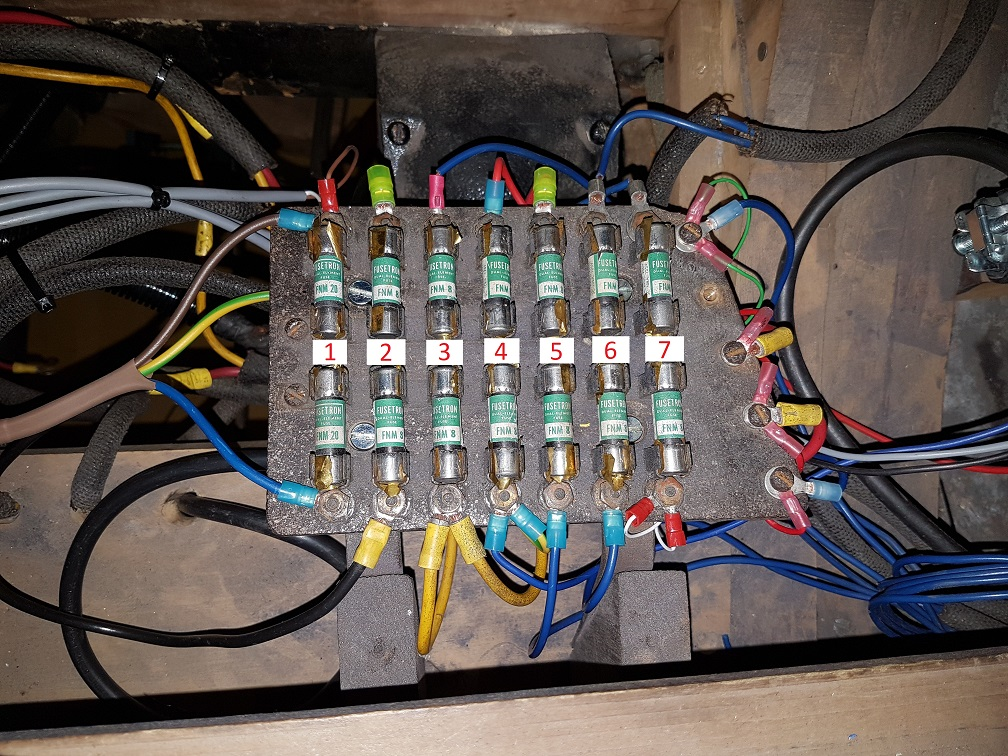
\includegraphics[width=0.8\textwidth]{images/Sicherungsbrett}
	\caption{Verdrahtetes Sicherungsbrett}
	\label{fig:Sicherungsbrett}
\end{figure}

\newpage
Dabei wird das 12 V jeweils unten und oben links eingespeist (auf Abbildung \ref{fig:Sicherungsbrett} Nummer 1). Somit ist + und - einzeln abgesichert. Jeder einzelne nachfolgende Abgang ist dann noch einmal separat jeweils + und - abgesichert. Diese Einspeisung, resp. Abgänge sind nachfolgend von links nach rechts aufgelistet:

\begin{compactitem}
\item Einspeisung 12 V (1)
\item Hupe (2)
\item Vorderlicht (3)
\item Blinker (ehemals Seitenlichter) (4)
\item Meterlicht (5)
\item Innenbeleuchtung (6)
\item Rücklicht (7)
\end{compactitem}

Nachfolgend wird kurz erklärt, was an den einzelnen Abgängen verändert wurde:
\begin{itemize}
\item Die Hupe wurde durch eine neuere ersetzt, da die alte nicht mehr funktionstüchtig war.
\item Die Vorderlichter wurden durch 12 V-LED-Scheinwerfer ersetzt. Dabei konnten die Lichter in die bestehenden Gehäuse eingebaut werden.
\item Die Blinker sind der wohl grösste Eingriff in die bestehende Verkabelung. Die Seitenleuchten werden durch Blinkerbirnen ersetzt. Zusätzlich wurde für den Blinkmechanismus ein Relais benötigt, welches sich unter dem Sitz befindet. Ebenfalls wurde unterhalb des Steuer- bzw. Richtungshebels ein Schalter mit drei Positionen (Nullzustand - Links - Rechts) installiert. Das gesamte Schema sieht dann wie folgt aus:

\begin{figure}[h]
	\centering
		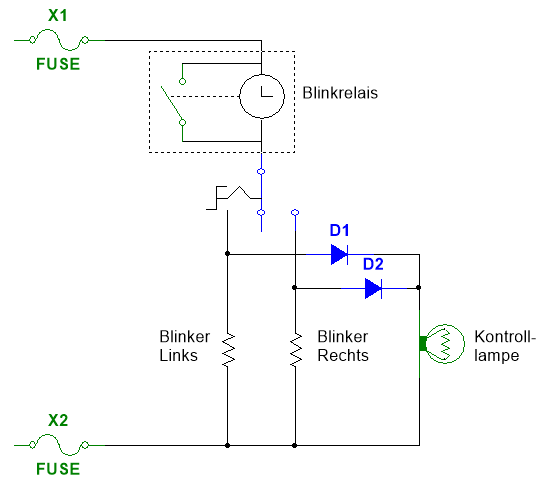
\includegraphics[width=0.6\textwidth]{images/Blinkerschaltung_Schema}
	\caption{Schema Blinkerschaltung}
	\label{fig:SchemaBlinkerschaltung}
\end{figure}

Die beiden Dioden D1 und D2 sind dafür zuständig, dass bei der Betätigung einer Blinkerrichtung zusätzlich nur die Kontrolllampe beginnt zu leuchten und nicht beide Blinker beginnen zu schalten.
\item Das Meterlicht bleibt gleich wie zuvor. Die Birne wurde durch eine baugleiche ersetzt.
\item Die Innenbeleuchtung konnte ebenfalls im Originalzustand belassen werden. Lediglich neue Birnen wurden eingesetzt.
\newpage
\item Das Rücklicht wurde ebenfalls überarbeitet. Das ursprüngliche Licht wurde am Fahrzeug belassen, ist jedoch nicht mehr im Betrieb. Zusätzlich wurden zwei 12 V-LED-Leuchten am Heck montiert. Diese sind fähig ein stärkeres Bremslicht und ein weniger starkes Standlicht zu betreiben. Um das Bremslicht zu betreiben, ist ein Endschalter am Bremspedal notwendig. Dieses wurde gemäss nachfolgendem Bild an der Stahlkonstruktion des Autos befestigt:

\begin{figure}[h!]
	\centering
		\includegraphics[angle=270,width=0.5\textwidth]{images/Bremspedal_Endschalter}
	\caption{Endschalter für Bremslicht}
	\label{fig:EndschalterBremslicht}
\end{figure}

Dieser Endschalter ist im aktiven Zustand, so wie es im Bild \ref{fig:EndschalterBremslicht} ersichtlich ist, offen und schliesst sich erst wenn die Bremse betätigt wird. Das Bremslicht ist immer aktiv. Das heisst auch wenn das Standlicht ausgeschaltet ist, funktioniert das Bremslicht autonom.

\end{itemize}

\newpage

Das Lichtschalterbrett wurde ebenfalls gemäss den Anforderungen der oben genannten Abgänge angepasst. Ersichtlich ist dieses Brett in der nachfolgenden Abbildung:

\begin{figure}[h!]
	\centering
		\includegraphics[width=0.5\textwidth]{images/Ansicht_Lichtschalterbrett}
	\caption{Ansicht des Lichtschalterbrettes}
	\label{fig:AnsichtLichtschalterbrett}
\end{figure}

Die Schalter sind wie folgt von oben nach unten den Abgängen zugeordnet und nummeriert:

\begin{enumerate}
\item Vorderlicht (1)
\item Unbenutzt (2)
\item Unbenutzt (3)
\item Meterlicht (4)
\item Innenbeleuchtung (5)
\item Rücklicht (6)
\end{enumerate}

\color{black}
\newpage